% !TEX root = ../thesis.tex
%
\setcounter{chapter}{1}
\chapter{Background}\label{chap:background}

\cleanchapterquote{If I have seen further, it is by standing on the shoulders of giants.}{Isaac Newton}{in a letter to Robert Hooke, 1675}

This chapter presents a survey of the relevant literature pertaining to the work carried out in this thesis. The research surrounding \ac{CT} is introduced, covering how the concept evolved and differentiated itself from \ac{CL}, the proposed definitions and ways it has been measured and supported so far. Furthermore, an introduction to \acp{TUI} is provided, suggesting how they can be used to aid learning and developing skills associated to \ac{CT}.

\section{Computational Thinking}
As discussed in the introduction, since the coming of the Information Age, technology has progressively taken on a more prominent role in our day-to-day life; from the simple task of turning on the engine of your car to the vastly more complicated process behind the management of a flight, it is unmistakably clear how much our entire society depends on software: technology surrounds every aspect of our lives, and relying on it so much can be daunting at times. Most people weren't born in a high-tech world such as the one we live in today, but rather saw it developing overtime during the course of their lives. They got generally familiar with digital systems through their adult life, rather than growing up in the digital age as the so-called Digital Natives.

Being computationally literate and knowing the way into technology --- and thus into our society --- are becoming much-needed skills to possess for an ever wider and heterogeneous audience. This explosion of interest is witnessed by the many public initiatives that have been quite successful in the past few years in promoting such skills, and even more are coming along following the same path: Code.org's Hour of Code~\cite{HOC} is the main example of a successful global initiative involving millions of students of different ages starting with 4-years old and aiming at introducing coding to a wide audience with different backgrounds. Many known figures have stressed the importance of possessing these skills: former President Obama pledged to provide \$4 billion in funding for \ac{CS} education in U.S. schools as part of the \ac{CS} for All initiative announced in 2016.

Many other initiatives and movements~\cite{Lee:2014er,Yadav:2014,Voogt:2015} are advocating the need of promoting coding and computational methods right from kindergarten and in disciplines outside \ac{CS} itself as a new form of literacy.

\subsection{Computational Literacy}
One of the pioneers of \ac{CT} is Seymour Papert, co-director of MIT Artificial Intelligence Laboratory from 1967 to 1981. He first mentioned \ac{CT} in his seminal 1980 book Mindstorms~\cite{Papert:1980uh}, where he discussed two aspects of computation, namely how it creates new knowledge, and how computers could be used to enhance thinking and change knowledge access patterns.

He connected \ac{CT} and digital pedagogy to a modern approach to education known as constructivism, a learning theory initiated by Jean Piaget~\cite{Piaget:1969vq}. Piaget was a developmental psychologist who often collaborated with Papert back in the 80s; in brief, he stated that learners construct new knowledge in their minds from the interactions of their experiences with previous knowledge. Papert developed his theory of constructionist learning on top of Piaget's constructivism by adding the notion that learning is enhanced when learners are engaged in ``constructing a meaningful product''.

In the introduction to Mindstorms, Papert refers to the widespread of personal computers, and how people imagined them permeating home life and businesses. But he was thinking beyond those roles, to ``how computers may affect the way people think and learn'':
\begin{quote}
  A few talked about the computer as a teaching machine. This book too poses the question of what will be done with personal computers, but in a very different way. I shall be talking about how computers may affect the way people think and learn. I begin to characterize my perspective by noting a distinction between two ways computers might enhance thinking and change patterns of access to knowledge.
\end{quote}

In the 1960s Papert, together with Bobrow, Feurzeig, and Solomon, presented LOGO~\cite{chakraborty1999logo}, one of the first high-level computer programming languages designed to embody constructionist principles. He continued to design and implement LOGO, creating what he deemed a social-constructionist sandbox. He believed that children are ``active builders of their own intellectual structures'', namely they could learn, apply, and come to know concepts and things through the process of writing programs: the ``child as epistemologist'', as he stated. Accordingly, he claimed that such material and symbolic activities fostered both \ac{CL} and conceptual skills, as the two are inseparable.

DiSessa~\cite{disessa2001changing} followed up on Papert's ideas on \ac{CL}, and better characterized \ac{CL} in comparison with the traditional meaning of \emph{literacy}, namely being able to read and write:
\begin{quote}
  Computers can be the technical foundation of a new and dramatically enhanced literacy, which will act in many ways like current literacy and which will have penetration and depth of influence comparable to what we have already experienced in coming to achieve a mass, text-based literacy. 
\end{quote}

He argues that literacy is built on three foundational pillars: first, the \textit{material} pillar, involves the external, materially based signs, symbols, depictions, or representations that are technologically based and designed (e.g., alphabet, grammar, and syntax for written language, numbers and symbols for arithmetic). The second pillar is \textit{mental or cognitive} and works in conjunction with the material basis of literacy to represent what we think and do with our minds in presence of materially based representations. The third pillar is \textit{social}, giving literacy a value within the community.

He focused on the material affordances of programming, claiming that it can turn into a literacy if it becomes infrastructural to everyday life; furthermore, he adds that its ease of use can be the key factor in whether it will indeed become infrastructural, using the example of Leibniz's more intuitive notation for calculus in comparison with Newton's.

\ac{CT} has a lot in common with DiSessa's definition of \ac{CL}, even though in a recent paper~\cite{disessa2018computational} he highlighted some key differences, indeed suggesting that the two movements should come together and join their current insights and future directions.

\subsection{Defining Computational Thinking}
After being mentioned a couple of times in Papert's work, \ac{CT} has been brought into the limelight more recently by Jeannette Wing in her 2006 seminal work~\cite{Wing:2006iz}. She reintroduced it as a mental skill set needed to solve complex problems like a Computer Scientist, but also widely applicable in today's information society.

At first, she did not mean to give a clear definition of \ac{CT} through a brief, summarizing sentence; on the contrary, she described its characteristics and how they can be exploited in everyday life. She argued that it is mostly about problem-solving, and enumerated a list of features typical of \ac{CT}, the most important being \emph{abstraction}, or the ability to think at different levels of abstraction: she stated that \ac{CS} is not programming, and thus that conceptualizing is key. She also referred to abstraction as a fundamental skill that has to be learnt by anyone to function in modern society, as opposed to a rote skill that is mechanical and repeated over and over. Indeed, in her vision Wing wished that \ac{CT} was part of the core teaching from the very young age, in the same way as reading, writing, and arithmetic are.

Four years later, Wing herself published another article~\cite{Wing:2010} in which she --- together with Jan Cuny of the National Science Foundation and Larry Snyder of the University of Washington --- provided a more precise and short definition:
\begin{quote}
  \ac{CT} is the thought processes involved in formulating problems and their solutions so that the solutions are represented in a form that can be effectively carried out by an information-processing agent.
\end{quote}

\ac{CT} is then both a thought process and a skill set. More precisely, it is regarded as the thought process involved in formulating problems and their solutions so that the ``solutions are represented in a form that can be effectively carried out by an information-processing agent''~\cite{Wing:2010}. Thus, Wing argues that \ac{CT} is mostly about problem-solving, as well as the capability of using abstraction, problem decomposition, and algorithmic thinking\deleted[comment={D2}]{ are regarded as highly relevant \ac{CT} skills}~\cite{Wing:2010,Voogt:2015,Moreno:2012}.

It covers far more than programming itself, including a range of mental tools reflecting fundamental principles and concepts of \ac{CS}, such as abstracting and decomposing a problem, identifying recurring patterns, and being able to generalize solutions. However, as also suggested by Wing's seminal work, \ac{CT} does not coincide with programming; rather, it ``includes a way of thinking about everyday activities and problems''~\cite{Shute:2017}. Such problems are often ill-structured (or wicked), in that they may have neither definitive formulation nor boundaries~\cite{Fischer:2017}, thus the ability to analyze and solve them is very useful in everyday life. In accordance with this view, Lu and Fletcher~\cite{Lu:2009} proposed to teach \ac{CT} by using languages based on notions that are familiar to people, rather than using programming languages; this way, concepts like abstraction and algorithmic thinking could be more easily brought about.

As highlighted in the recent review by Shute et al.~\cite{Shute:2017}, there is little agreement on the exact definition of \ac{CT} and over the years several different definitions have been proposed.

Most of the literature works attempt to define \ac{CT} skills as a set of facets comprising abstraction, algorithmic thinking, problem decomposition, and debugging. Shute et al.~\cite{Shute:2017} add iteration and generalization as two more skills that are important in \ac{CT}.

\textit{Abstraction} is the ability to think at different levels and the capability of modelling the core aspects of problems/systems by discarding irrelevant details~\cite{Wing:2006iz}. Abstraction helps modelling problems and systems by capturing only the essential properties common to a set of objects\replaced[comment={D3}]{; it allows hiding non-relevant differences, out of the scope chosen to evaluate the problem context}{ while hiding their differences, the latter is not relevant from the perspective chosen to evaluate the context}. Building systems in terms of layers of abstraction allows developers to focus on one layer at a time and only on its formal relations between its adjacent layers; when moving to a higher-level, there is no need to worry about the details of the underlying specifications, thus providing us with an easy and effective way of focusing on one issue at a time without forgetting the overall process.

\textit{Problem decomposition} is concerned with breaking a problem down into manageable units~\cite{Wing:2006iz}. It is used when breaking problems, algorithms, artefacts, processes, and systems down to their functionalities, thinking about them in terms of their parts. Their components can then be understood, solved, developed, and evaluated separately, making complex problems easier to solve and large systems easier to design.

\textit{Algorithmic thinking} refers to the ability to create procedures as ordered steps to implement solutions~\cite{Atmatzidou:2016}.

\textit{Debugging} is particularly emphasized in~\cite{Bers:2014fk} as the ability to identify and fixing errors when algorithms do not provide the expected solution.

According to~\cite{Shute:2017}, \textit{iteration} is important for repeating design processes to refine solutions and \textit{generalization} is fundamental to transfer \ac{CT} skills to a wide variety of contexts.

In 2013 Selby and Woollard published an important work~\cite{eps346937} which surveyed publications related to \ac{CT} and the definitions extended from Wing's original one. They discussed the need for a precise definition, presenting support from the literature and the academic community. They found that the most common terms used to define \ac{CT} are ``a thought process'', ``abstraction'', and ``decomposition''. Some other terms relate to different sets of thinking skills like logical, mathematical, and engineering thinking, problem-solving terms, and other \ac{CS} terms. They propose a definition which states that \ac{CT} is an activity, often product oriented, associated with, but not limited to, problem-solving. It is a cognitive or thought process that reflects:
\begin{itemize}
  \item the ability to think in abstractions,
  \item the ability to think in terms of decomposition,
  \item the ability to think algorithmically,
  \item the ability to think in terms of evaluations, and
  \item the ability to think in generalisations.
\end{itemize}

Starting from Wing's definition, Repenning and his colleagues from the University of Colorado modelled \ac{CT} as an iterative process structured in three stages~\cite{Repenning:fy} (see Figure~\ref{fig:ctiterative}):
\begin{enumerate}
  \item \textit{problem formulation (abstraction)}, namely a verbal or diagrammatic conceptualization of the problem, in which abstraction plays a fundamental role to conceptualize a problem. Usually, a form of visual thinking can be helpful (e.g., diagrams);
  \item \textit{solution expression (automation)}, where the solution is described in a non-ambiguous way so that it can be executed by a computer. The most important tool in this stage is programming;
  \item \textit{execution and evaluation (analysis)}, where one may obtain visualizations of the outcome from the other two stages and evaluate them.
\end{enumerate}

On the basis of the evaluation, problem formulation could be refined, and the cycle starts again. The idea they proposed is that the three stages of the \ac{CT} process should be supported and integrated by means of \ac{CT} tools, such as any kind of programming --- including \ac{EUP} --- but also informal drawings, mind maps, and task-specific languages.

\begin{figure}[ht!]
  \centering
  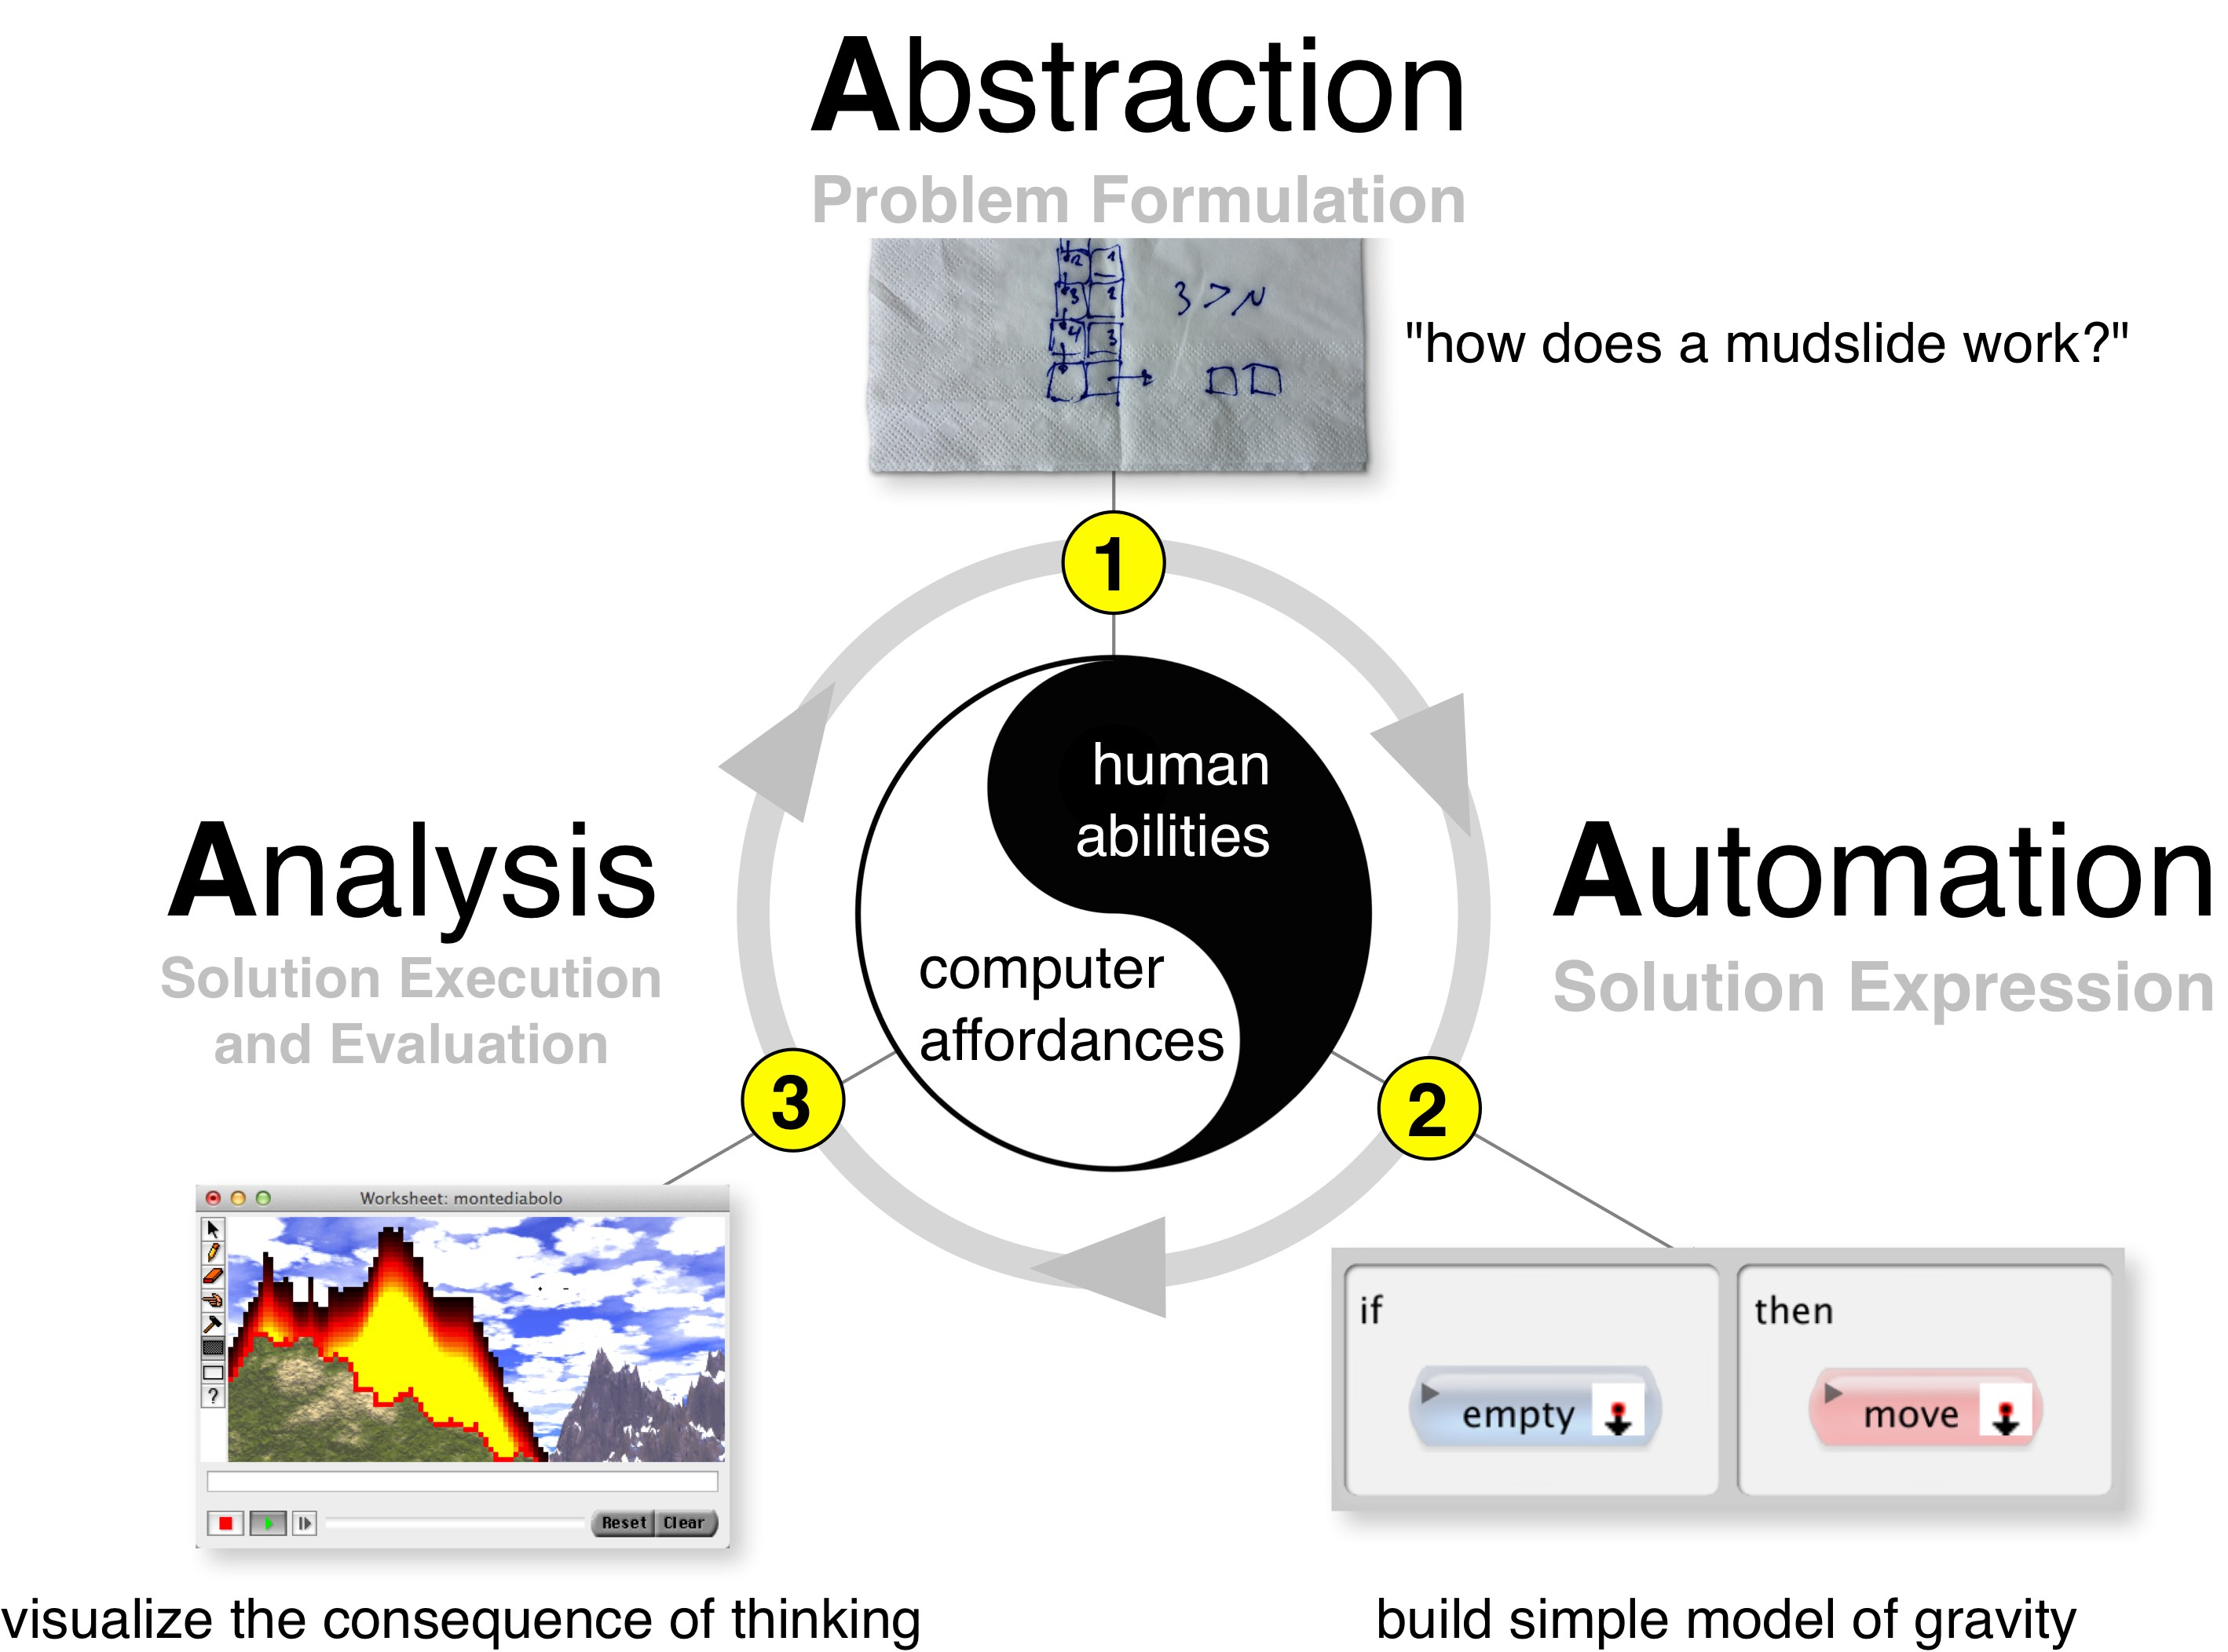
\includegraphics[width=0.75\textwidth]{images/c2/CTIterative.jpg} 
  \caption{The iterative \ac{CT} proc\-ess di\-vid\-ed in\-to three stages, shown through the ex\-am\-ple of a mud\-slide sim\-u\-la\-tion~\cite{Repenning:fy}.}\label{fig:ctiterative}
\end{figure}

The whole process is iterative since the third stage often exposes the flaws of the previous two steps and it requires to start again from the beginning. Describing the process in this way allows to point out the different responsibilities at each stage: execution and evaluation are entirely performed by a computer, while the phase of solution expression lies in the hands of the user. Repenning notes that contrarily to what one might think, the workload of the problem formulation stage can be shared between human and computer, the latter providing useful tools to support the conceptualization process.

\replaced{Another popular framework attempting to define \ac{CT} was proposed by Brennan and Resnick in 2012~\cite{Brennan:2012}: t}{This viewpoint about \ac{CT} is much different from the one Brennan and Resnick embrace in their 2012 paper~\cite{Brennan:2012}. T}heir approach is based on a three-dimensional framework composed of computational Concepts, Practices, and Perspectives. Concepts refer to typical programming features and structures, such as sequences, loops, parallelism, events, conditionals, operators, and data. \ac{CT} Practices are \replaced{related to how people learn and put these concepts into practice}{about how the user learns and puts into practice these concepts}. \replaced{They}{Brennan and Resnick} identified four practices:
\begin{enumerate*}[label=(\arabic*)]
  \item being incremental and iterative,
  \item testing and debugging,
  \item reusing and remixing,
  \item and abstracting and modularizing.
\end{enumerate*}
\replaced{Finally,}{The} computational Perspectives try to describe how the human\deleted[comment={D4}]{’s} mind changes the way it views the world when experiencing \ac{CT}. For in\-stance, com\-put\-ing devices can be considered as something to be consumed, but for computer scientists they are also powerful tools for designing and expressing themselves. Social practices are affected as well because the opportunity of communicating \added{and collaborating }with people from all over the world brings huge benefits. It becomes possible to cooperate at a distance, but also to access and contribute to an unbelievable amount of shared knowledge. The last of these perspectives is the so-called questioning, described as \deleted{the habit of }not taking anything for granted and using design as a mean\deleted{s} to overcome obstacles. It might be the case of an open software with a limited or missing feature; a possible reaction might be to fix it or add it to the program.

\replaced[comment={MP2}]{This definition evolved after years of work with Scratch~\cite{Resnick:2009bd}, a block-based \ac{VPL} designed to introduce programming to people --- children in particular --- as well as allow them to develop always more complex projects. Therefore Brennan and Resnick's definition is directly linked to the tools designed to foster \ac{CT} and provides a way to analyse them at different but complementary levels}{This definition of \ac{CT} is tailored to developers, programmers and computer scientists in general. It is worth noting indeed that Brennan and Resnick introduced this definition after years in which they organized Scratch workshops and studied the activity of the Scratch online community. Scratch~\cite{Resnick:2009bd} is a block-based \ac{VPL} designed to introduce programming to people --- children in particular --- but on the other side, it has a really high ceiling, as it allows to develop also complex projects. Basically, Brennan and Resnick formulated their framework for \ac{CT} by observing the actions of people involved in programming, precluding from their analysis any other activities}.

\replaced{Another}{A third} viewpoint of \ac{CT} which contains a bit of both the definitions above, is the one by Kazimoglu et al.~\cite{Kazimoglu:2012ft}. They identified five core skills as a result of an analysis of existing studies, before developing a computer game, Program Your Robot, which has the aim of teaching \ac{CT} through programming, though at a higher level than Scratch. The core skills are problem-solving, building algorithms, debugging, simulation, and socializing. It is interesting that this set \replaced{strives}{seems} to summarize and blend Wing's and Brennan and Resnick's approaches\replaced{, thus it pulls the original \ac{CT} definition more towards programming concepts, and the latter to a higher level}{. This last definition appears to be the most complete and balanced since it features skills that can be owned by anybody, such as problem-solving and socializing, but also others more related to programming}.

Finally, a systematic literature review published in 2016 by Kalelioglu et al.~\cite{kalelioglu2016framework} analysed the many existing definitions of \ac{CT} and argued that, even though many common characteristics can be found across different papers trying to define \ac{CT}, the research is still at an early stage of maturity, and not many present solid theoretical or conceptual backgrounds. They propose a five stages framework based on the surveyed papers that combines both the scope of \ac{CT} and problem-solving, but even this definition is not yet finalised and still in the development phase.

However, in the past few years, some critiques around the concept of \ac{CT} have also been published: in their work~\cite{tedre2016long}, Tedre and Denning critically analyse the research surrounding \ac{CT} and put it in perspective with the previous research from the 80s of computing in education. They hold a critical view of the \ac{CT} buzz, arguing that much research has already been carried out in the past two decades under different definitions, and \ac{CT} risks of failing in the same ways the previous research wave has. The risks for the \ac{CT} research community are to fall into the trap of reinventing the wheel and water down 80s initiatives, considering \ac{CT} as the best way of thinking in all environments, which is an oversimplification.

Lorena A. Barba~\cite{CTLAB2016} wrote a blog post in 2016 that generated a lot of discussion within the \ac{CT} research community, entitled ``Computational Thinking: I do not think it means what you think it means''. She rejected the idea that \ac{CT} means thinking like a Computer Scientist and is not about programming, arguing that current definitions are moving away from the initial ideas of Papert, by putting emphasis on problem-solving rather than projects, understanding rather than doing, content priming over media, and operations over their objects representations. She also argued that abstraction is not unique to \ac{CS} and many other ideas of CS are not involved by current definitions. She suggested that by applying more closely original Papert's ideas like relevant projects, socializing, and investing on the social and cultural contexts might increase the fun of CS courses and making them less scary.

As remarked by the many studies reported, more research is definitely needed on developing a working definition of \ac{CT} and the skills it encompasses\added[comment={MP2}]{; for the scope of this thesis though, Brennan and Resnick's proposed framework~\cite{Brennan:2012} represents the most complete and directly observable definition to be exploited when designing a new \ac{CT} tool, as reported in the next section}.

\subsection{Measuring Computational Thinking}
As a consequence of being a recent topic, the assessment of \ac{CT} skills is still in a very early and experimental stage. There are some intrinsic problems that must be still overcome. First of all, the lack of a unique definition of \ac{CT} skills implies that the choice of the method for the evaluation strictly depends on which skills are considered as pivotal\added{, thus the assessment framework directly depends on the definition employed}. Moreover, it is difficult to identify an evidence-centred way of assessing abilities like problem-solving or abstraction.

A very interesting mapping study has been carried out in 2016 by de Araujo et al.~\cite{de2016systematic} in which they gathered data from 27 studies performed in educational environments published between 2009 and 2016. They questioned \deleted{about }the approaches used in promoting \ac{CT}, which skills were assessed, and what instruments or artefacts were used.

The most widespread approach among these studies is represented by workshops, modules, and regular classes (13 out of 27), followed by exams without any classes (6), and frameworks specifically designed for assessing \ac{CT} skills (5). Only three studies involved games or online interactive platforms. For what concerns the \ac{CT} skills evaluated, problem-solving, algorithm construction, and abstraction are the only ones that can be considered recurrent, being involved in respectively 26, 20, and 9 studies; other abilities are not mentioned by more than 4 studies, witnessing the high uncertainty in establishing a common definition for \ac{CT}.

The most popular tool employed to assess \ac{CT} skills is multiple-choice questionnaire, found in 11 studies. Other very spread instruments are code evaluation (10 studies), and responses (9), while surveys, interviews, games, videos, lesson plans, and design scenarios are very rarely used (9 times in total).

\replaced[comment={MP2}]{The most common way of assessing \ac{CT} skill progression is through the analysis of the produced artefacts; this usually leads to a checklist-based evaluation, consisting of}{When \ac{CT} skills are fostered through programming courses, analyzing the code is the most common way of assessing the progress of the student. However, this approach leads to a limited evaluation, based on checklists. It basically consists of} an automated analysis looking for the presence of \replaced{constructs}{blocks} (e.g., if or while conditions), making it suitable for assessing the so-called \ac{CT} Concepts, as defined by Brennan and Resnick~\cite{Brennan:2012}. Clearly, it gets quite difficult to measure how developed Practices and Perspectives are; this is why when evaluating the impact of \replaced{a new tool}{Scratch} over users' \ac{CT} skills, they also introduced artefact-based interviews and design scenarios in their assessment approach\added{, as summarised in table \ref{tab:reis}}. The interviews try to explore how the users developed the discussed artefact, questioning also about their background, how and if they participate in the online community and what is their general opinion about a tool. However, \replaced{as recognized by the authors, no single approach is sufficient to capture all nuances of \ac{CT}, an a combination of approaches could be appropriate}{the authors recognize that perspectives (expressing, connecting, and questioning) are very hard to assess, even on this three-way evaluation}.

\begin{table}[ht!]
  \caption{Strengths and limitations of different assessment approaches as summarised by Brennan and Resnick with respect to their \ac{CT} framework~\cite{Brennan:2012}.}\label{tab:reis}
  \centering
  \begin{tabular}{M{0.13\linewidth}m{0.245\linewidth}m{0.245\linewidth}m{0.245\linewidth}}
    \toprule
    & \textit{Concepts} & \textit{Practices} & \textit{Perspectives} \\
    \midrule
    \textit{Project Analysis} & Com\-mands cor\-re\-spond to con\-cep\-tu\-al en\-coun\-ters. & \multicolumn{1}{c}{---} & Pos\-si\-bly add\-ing ex\-tra me\-ta-da\-ta for off\-line a\-nal\-y\-sis. \\
    \textit{Artefact-Based Interviews} & Nu\-ances of con\-cep\-tu\-al un\-der\-stand\-ing, but with limited set of projects. & Based on own au\-then\-tic de\-sign ex\-pe\-ri\-ences, but lim\-it\-ed by mem\-o\-ry. & Maybe, but hard to ask directly. \\
    \textit{Design Scenarios} & Nu\-ances and range of con\-cep\-tu\-al un\-der\-stand\-ing, but externally selected projects. & Real-time and in novel situation, but externally selected projects. & Maybe, but hard to ask directly. \\
    \bottomrule
  \end{tabular}
\end{table}

If the considered \ac{CT} skills belong to a higher level than programming, it becomes almost impossible to rely on quantitative data; for this reason, assessors usually recur to interviews and surveys. For instance, in order to evaluate the Program Your Robot game~\cite{kazimoglu2012serious}, the authors asked students to give feedback about the gameplay and their experience, highlighting when a \ac{CT} skill had been stimulated in a participant.

Atmatzidou and Demetriadis~\cite{Atmatzidou:2016}, authors of the educational robotics course mentioned in the previous section, asked participants to answer two intermediate questionnaires, in which they tried to investigate how \ac{CT} skills were evolving in the activity of programming robots. Students were also prompted to give more personal views about the understanding of \ac{CT} concepts in a questionnaire after the completion of the training. Besides, a think-aloud protocol was applied when students were asked to solve a programming task, followed by an interview in which opinions on the whole course were collected.

A similar approach was followed by the authors of CTArcade~\cite{Lee:2014er} when trying to compare how the paper and the software version of tic-tac-toe affected algorithmic thinking, pattern decomposition, pattern recognition, and abstraction. Interviews and think-aloud protocol were used, as well as a deep analysis of the users’ gameplay guided by a codebook for retrieving instances of the considered \ac{CT} skills.

More generally, as de Araujo et al.~\cite{de2016systematic} pointed out, different interpretations of \ac{CT} skills and concepts deeply impact their assessment, leading to different approaches, metrics, and dimensions used in experiments.\added[comment={MP2}]{ Therefore, in order to properly address the Research Question posed by this thesis, a combination of different approaches will be used --- as suggested by Brennan and Resnick~\cite{Brennan:2012} --- in order to try to capture most of the \ac{CT} different dimensions summarised in table \ref{tab:reis}.}

\subsection{Fostering Computational Thinking}
Even though \ac{CT} was widely discussed for the first time only a few years ago, there have been attempts to foster it starting from the 1960s. \replaced[comment={D5}]{Programming has proven to be an excellent way of developing \ac{CT} skills~\cite{Orr:2009ip}, thus}{Since \ac{CT} and programming are related, any attempt of} teaching how to program can also be considered as an attempt to embolden the development of \ac{CT} skills. This is the reason why the very first effort to teach \ac{CT} can be attributed to Seymour Papert and Wally Feurzeig, who designed and developed the LOGO programming language in 1967~\cite{chakraborty1999logo}. It was an adaptation of the functional programming language Lisp and the target users were specifically children, with the aim of teaching them the basic concepts of programming.

Afterwards, in the 1980s programming games appeared. The basic idea is to make programming more desirable and enticing adding the possibility of letting your program ``compete'' against others’. RobotWar~\cite{ROBOTWAR}, published in 1981, uses a language similar to BASIC, which was praised for being easy to learn. Players develop a program that simulates the behaviour of a robot, which then competes against multiple opponents in an arena. A few years later, Crobots~\cite{CROBOTS} was released; it was based on a reduced version of C, and programs were written by the users in order to seek out and destroy other robots.

Game design represents a more recent approach to teaching programming and \ac{CT} skills. In 1996 AgentSheets~\cite{Repenning:2000}, designed by Repenning, was released, even though the first prototype dates back to 1989. AgentSheets is still used in multiple contexts, from middle to high schools to academic environments, for various purposes such as introducing to programming, supporting storytelling, and prototyping simple games, just to name a few. The tool takes its name from the fact that the user develops the program on a grid resembling a spreadsheet, whose cells contain agents (see Figure~\ref{fig:agentsheets}). These entities, visualized as pictures, can perform multiple actions like reading Web pages and playing sounds and animations. Drag-and-drop interaction is \replaced[comment={D6}]{employed to support users}{supported, which revealed to be an interaction style suitable to people} without any programming background.
\begin{figure}[ht!]
  \centering
  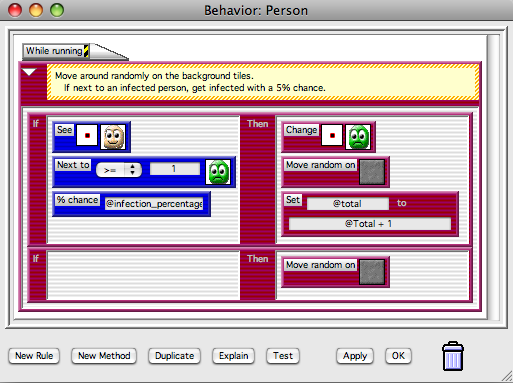
\includegraphics[width=0.75\textwidth]{images/c2/AgentSheets.png} 
  \caption{Example of the definition of an agent in AgentSheets.}\label{fig:agentsheets}
\end{figure}

The drag-and-drop paradigm is provided also by Alice~\cite{Herbert:2012}, developed at the Carnegie Mellon University starting from 1997. Alice is actually an object-based programming language that allows creating animations, with an integrated development environment that allows users to forget the language syntax. Therefore, Alice is a valid tool for supporting storytelling while being exposed to basic programming concepts without the burden of remembering syntactic constructs.

Perhaps the most influential and versatile tool for learning how to program is Scratch~\cite{Resnick:2009bd}, developed at the MIT and publicly released for the first time in 2005. It is a \ac{VPL} whose interaction is made simple thanks to draggable instructions represented by blocks, fitting one another like puzzle pieces (as shown in Figure~\ref{fig:scratch}). The process of assembling instructions is guided by the different shapes and colours of the blocks, suggesting which constraints must be satisfied. One of its biggest strengths is the large and heterogeneous community of users that, combined with the possibility of reusing and remixing other users' code, allows to cooperate, share knowledge, and realize complex projects easily. The popularity of Scratch increased in the UK when Code Club~\cite{CODECLUB} was founded in 2012, an initiative that aims to develop coding skills in children teaching the Scratch language itself, but also HTML, CSS, and Python.

Program Your Robot~\cite{kazimoglu2012serious} is a recent game prototype developed by the research group led by Kazimoglu and colleagues, cited in the previous section. Based on the five core skills they identified as fundamental for \ac{CT}, they developed a puzzle solving game in which the player has to assist a robot reaching a certain point on a grid. The robot will follow very simple instructions given in the form of an algorithm, while the score depends on conditions, for example, if two functions have been declared and then called by the algorithm. It differs from the software applications mentioned before, since they can be deemed programming languages at all effects, while Program Your Robot is conceived as a serious game. But most of all, tools like Scratch were designed in order to teach the basics of programming and to show how fun it can be. Instead, Kazimoglu and his colleagues were moved by the goal of producing a game that could explicitly foster \ac{CT} skills.
\begin{figure}[ht!]
  \centering
  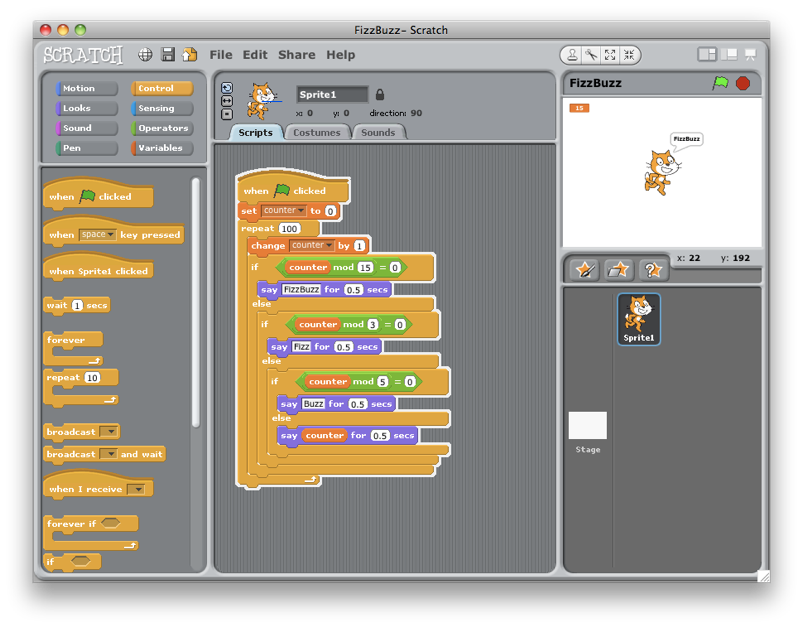
\includegraphics[width=0.75\textwidth]{images/c2/Scratch.png} 
  \caption{An example of a program written with Scratch.}\label{fig:scratch}
\end{figure}

CTAarcade~\cite{Lee:2014er} is another serious game, designed with the target of boosting \ac{CT} in players by letting them formalize their tacit knowledge and make a step towards abstraction. In CTAarcade users have to implement a set of rules that are observed by a character while playing Tic-Tac-Toe. Making these rules explicit is considered a very important process because they can often be applied in a natural, perhaps unconscious way and normally there is neither occasion nor reason to transform this knowledge into abstract instructions.

Another very interesting approach at fostering \ac{CT} has been explored by Atmatzidou and Demetriadis in 2016~\cite{atmatzidou2016advancing}, through seminars and sessions on educational robotics. Students aged 15 and 18 participated in a study in which they were exposed to notions that gradually became more and more complex, from basic programming concepts to managing sensors and variables, trying to put into practice what has been taught during the seminars. It emerged that programming robots actually helped to develop \ac{CT} skills (abstraction, generalization, algorithm construction, modularization, and decomposition capabilities were assessed), regardless of age.

In the next section, a survey of \acp{TUI} literature is presented, together with an overview of their benefits on learning as support for the original claim of using them to foster \ac{CT} skills.

\section{Tangible User Interfaces}\label{sec:tuirw}
Declining hardware costs have recently enabled many new technologies to be available to a wider audience, together with new and engaging interaction modalities, particularly using gestures or object movements; this revolutionary paradigm goes under the name of the \ac{NUI}, and it allows people to act and communicate with digital systems in ways to which they are naturally predisposed.

The term \textit{natural} has been used in a rather loose fashion, meaning intuitive, easy to use or easy to learn; many studies argue that natural interaction can be designed either by mimicking aspects of the real world~\cite{Jacob:2008dj} or by drawing on our existing capabilities in the communicative or gesticulative areas~\cite{Wigdor:2011:BNW:1995309}.

One of the most successful and developed approaches falling into the first category has been introduced by Ishii and Ullmer~\cite{Ishii:1997gy} and is known as \acp{TUI} (see Figure~\ref{fig:reactable} for an example). The aim of \acp{TUI} is to give bits a directly accessible and manipulable interface by employing the real world, both as a medium and as a display for manipulation; indeed by connecting data with physical artefacts and surfaces bits can be made tangible.

Using physical tokens as interfaces to computer systems was pioneered by Fitzmaurice and Buxton~\cite{fitzmaurice1997graspable} with Graspable User Interfaces: they build on the intuitive knowledge people have of everyday objects and take advantage of their rich physical affordances. They provide a tight match between real and digital objects through their similarity in terms of physical shape or types of manipulations that can be applied to them.

\begin{figure}[ht!]
  \centering
  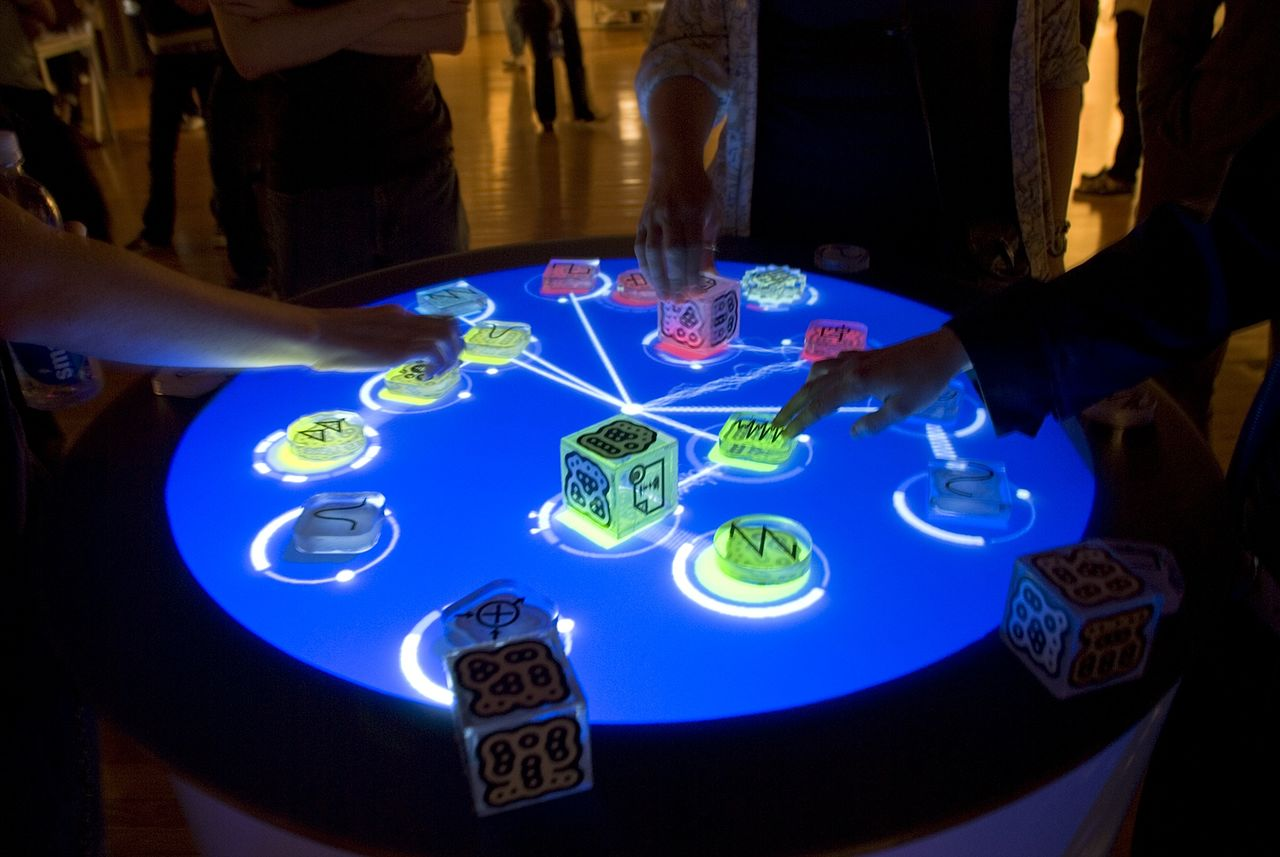
\includegraphics[width=0.75\textwidth]{images/c2/Reactable.jpg} 
  \caption{Reactable, an electronic musical instrument with a tabletop \acf{TUI}~\cite{jorda2007reactable}.}\label{fig:reactable}
\end{figure}

Many studies in this research area investigate the supposed benefits offered by this interaction paradigm, ranging from intuitiveness~\cite{Ishii:1997gy}, experiential learning through direct manipulation~\cite{Manches:2009kg, Parkes:2008bu}, motor memory~\cite{Weiss:2009ct}, accuracy~\cite{Muller:2014kx}, and collaboration~\cite{Subramanian:2007kx}. Furthermore, the effects of employing a \ac{TUI} to interact with a digital system are certainly dependent on the tasks and domain, as many comparative studies suggest~\cite{Weiss:2009ct, Muller:2014kx, Hancock:2009bg}; for this reason, Kirk et al.~\cite{Kirk:2009ue} made the case for hybrid surfaces, employing physical elements together with digital ones.

Researchers are also debating how em\-ploy\-ing \acp{TUI} re\-flects on learn\-ing~\cite{Horn:2009be,Marshall:2007dr,Antle:2013ho}, with spe\-cif\-ic ref\-er\-ence to highly abstract concepts: this stems from Piagetian theories~\cite{Piaget:1969vq} supporting the development of thinking --- particularly in young children --- through manipulation of concrete physical objects. Other studies~\cite{Wang:2014jy,Horn:2011ch} are even linking this effect to the development of \ac{CT} skills~\cite{Wing:2006iz}, namely a new kind of analytical thinking integral to solving complex problems using core computer scientists' tools, such as abstraction and decomposition.

\section{Contributions}
\added[comment={MP6}]{The Literature Review described in section \ref{sec:tuirw} has been previously published in~\cite{Turchi:2015dr,Turchi:2015kr,turchi2017tapas}.}

\section{Conclusion}
In this chapter, a literature review on \acl{CT} research has been presented, starting from how the concept evolved from \acl{CL}, its many proposed definitions and ways it has been evaluated so far. Furthermore, an introduction to \acp{TUI} has been presented, suggesting the many ways they can aid learning and developing skills associated with \acl{CT}.

The next chapter starts the investigation on the effects of tangible interaction on the development of \ac{CT} skills and focuses on existing tools used in education and their effects on promoting them.